\chapter{Introduction}\label{ch:intro}

% **************************** Define Graphics Path **************************
\ifpdf
    \graphicspath{{figures/chapter1-figs/}{Chapter1/Figs/PDF/}{Chapter1/Figs/}}
\else
    \graphicspath{{Chapter1/Figs/Vector/}{Chapter1/Figs/}}
\fi

\section{The Necessity of Fundamental Symmetry Violations}

The theoretical prediction \cite{Dirac1928, Dirac1930, Oppenheimer1930, Dirac1931} and experimental discovery \cite{Anderson1932, Anderson1933} of the existence of antimatter has been one of the most monumental advancements of modern physics. Apart from the detection in cosmic rays \cite{Anderson1932, Anderson1933, Blackett1933} and creation in the Berkeley Lab's Bevatron \cite{Chamberlain1955}, not much was known about the reasons for the gross lack of antimatter in the universe. However, the observations of Parity (P) \cite{Wu1957, Garwin1957} and Charge-Parity (CP) \cite{Christenson1964} violations alluded to the possibility that perhaps fundamental symmetry violations during the creation of the universe may have played a role in the dominance of matter over antimatter. To explain the origin of the known universe, the Big Bang hypothesis was proposed \cite{ Friedman1922, Lemaitre1927, Bartelmann2010} and later supported by the observation of the accelerated expansion of the universe \cite{Hubble1929, Bartelmann2010} and the Cosmic Microwave Background (CMB) Radiation \cite{Penzias1965, Dicke1965, Bartelmann2010}. It became apparent that during the hot and dense stage of the earliest universe \cite{Gamow1946, Alpher1948, Bartelmann2010}, matter and antimatter initially existed in creation-annihilation equilibrium, however, as the universe cooled off over time, only a small amount of matter remained, making up the universe observed today. From the observations of Big Bang Nucleosynthesis and the CMB \cite{Fields2020, PDG2022, Bartelmann2010}, this matter-antimatter asymmetry or the baryon asymmetry, $\eta$, of the present universe has been measured as: 
\begin{equation}
    \eta = \frac{n_B - n_{\Bar{B}}}{n_{\gamma}} = 6.14(19) \times 10^{-10}
\end{equation}
This smallness of $\eta$ confirms the dominance of matter in the presently observed universe as compared to the early universe. Furthermore, the Alpha Magnetic Spectrometer-01 measured a null result at the level of $10^{-6}$ in its search for antimatter counterparts of Big Bang light nuclei \cite{Alcaraz1999}, and is expected to further constraint this result from the Alpha Magnetic Spectrometer-02, currently taking data on the International Space Station \cite{Kounine2012}. Despite all these observations, the underlying fundamental mechanism responsible for this baryogenesis is still unknown.

To provide an explanation, Sakharov postulated a set of criteria \cite{Sakharov1991} required by the observed baryon asymmetry:
\begin{enumerate}
    \item The first criterion is the presence of a baryon number, $B$, violating interaction. The baryogenesis mechanisms must be able to convert antimatter i.e. $ B  = -1$  into matter i.e. $ B  = 1$ or vice versa, corresponding to a baryon number violation by going from $ \Delta  B  = 0$ to $ \Delta  B  \neq 0$.
    \item The second criterion is the departure of baryogenesis from thermal equilibrium. Under thermal equilibrium, the baryogenesis mechanism will cause the universe to eternally oscillate between the matter and antimatter state, assuming degeneracy under Charge, Parity \& Time -Inversion (CPT) invariance. Therefore, baryogenesis must have been operating under non-equilibrium conditions.
    \item The third criterion is that baryogenesis must be a CP violating mechanism and favor the production of matter over antimatter. Otherwise, equal amounts of matter and antimatter would have been created and annihilated with no net effect.
\end{enumerate}

The Standard Model (SM), does satisfy the first of Sakharov’s conditions via the sphaleron mechanism \cite{Kuzmin1985, Hooft1976}. Although possible in the early hot universe, this mechanism is predicted to exist at energies of several tens of TeV, and so far has not been observed in any experimental setting. The SM does not satisfy the second condition since the observed mass of the SM predicted Higgs like particle discovered at LHC is much larger \cite{Sirunyan2020} and prefers a smooth crossover rather than a CP-violating and baryon number violating phase transition needed to cause a deviation from thermal equilibrium \cite{Morrissey2012}. The third condition is allowed by the CP violating phase of the CKM matrix \cite{Kobayashi1973} but due to insufficient observations of CP violation so far, the SM is not enough to satisfy this condition either. Based on this, it is extremely improbable that the SM at the electroweak scale was responsible for baryogenesis introduced to explain the baryon asymmetry \cite{Canetti2012, Morrissey2012, Dine2003}. Therefore, searches for beyond the SM physics will lead to a greater understanding of the early formation of our universe.

Experimental searches for CP violation open a promising route towards BSM physics, which may explain the cosmic baryon asymmetry \cite{Morrissey2012, Bigi2009, Sozzi2008}. Within the Standard Model, CP symmetry is broken by the complex phases in the flavor changing charge current weak interactions arising from the Yukawa couplings of the Higgs scalar field to the quarks \cite{Kobayashi1973}. BSM physics may introduce new coupling and interactions that can enhance the CP violations beyond the level of the SM \cite{Bigi2009, Sozzi2008}.

\afterpage{
\begin{figure}
    \centering
    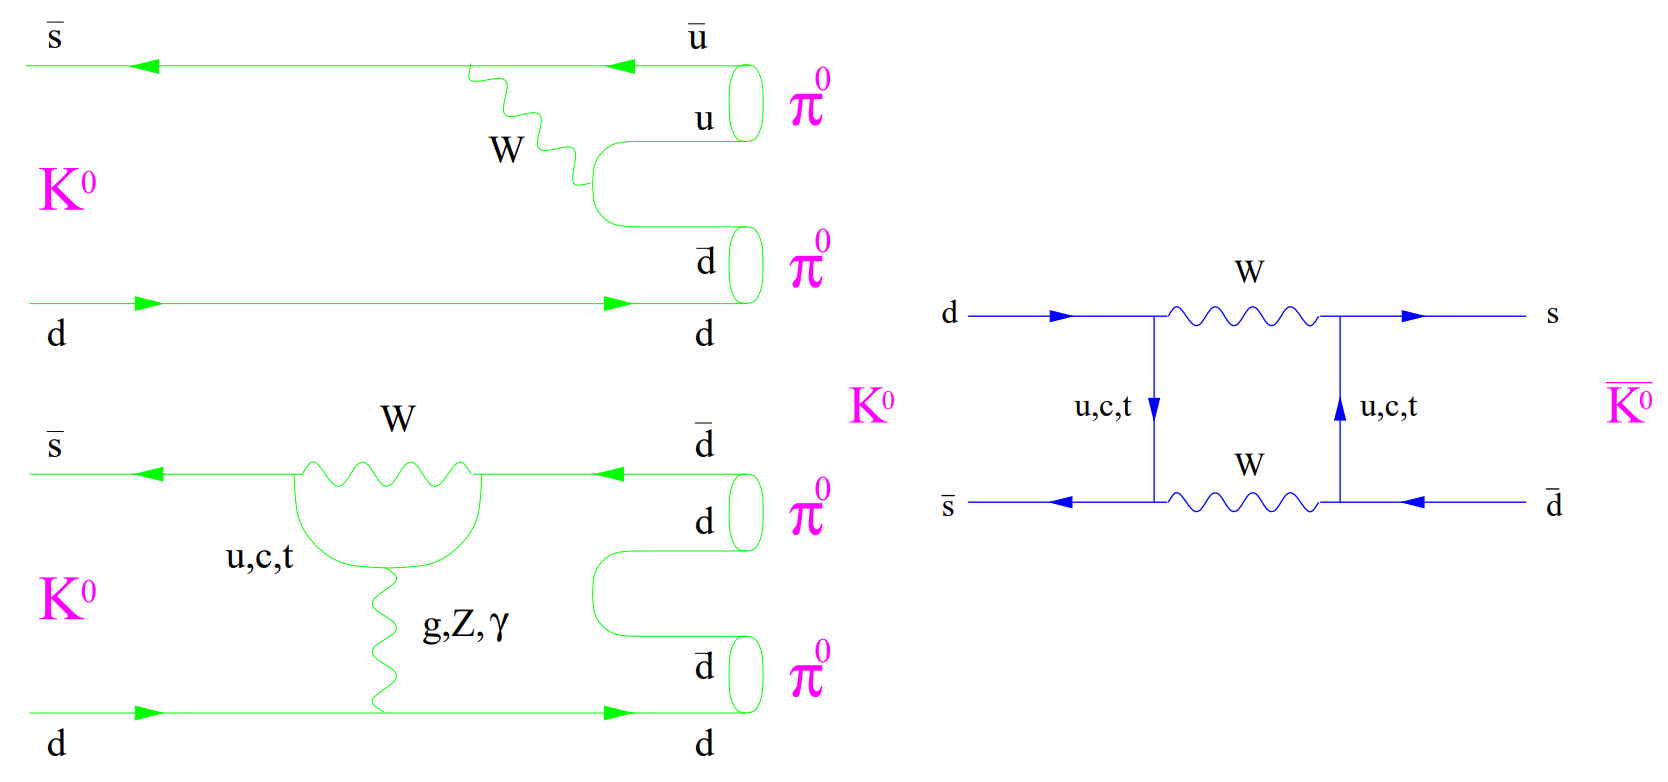
\includegraphics[width=\textwidth]{figures/chapter1-figs/Kaon_CPviolation.png}
    \caption[The left figure shows the “tree” level (top) and “penguin” level (bottom) diagrams responsible for the direct CP in Kaon decays. The right figure shows the “box” level diagrams responsible for the indirect CP in neutral Kaon mixing.]{The left figure shows the “tree” level (top) and “penguin” level (bottom) diagrams responsible for the direct CP in Kaon decays. The right figure shows the “box” level diagrams responsible for the indirect CP in neutral Kaon mixing. Figure taken from \cite{Sozzi2008}.}
    \label{fig:Kaon_decay}
\end{figure}
\clearpage}

The first evidence of CP violation was discovered by the observation of neutral Kaon decay, $K_L^0 \rightarrow \pi^+ \pi^-$, in 1964 \cite{Christenson1964}. This indirect CP violation was attributed to the fact that $K_L$ and $K_S$ mass eigenstates are a mixture of CP even and odd weak flavor eigenstates arising from ``box" type interaction diagrams as shown in \cref{fig:Kaon_decay} \cite{PDG2022, Bigi2009, Sozzi2008}. Direct CP violation was also discovered in the direct Kaon decays, where a tiny difference of $\left( 1.6 \pm 0.2 \right) \times 10^{-3}$ between the observed decay amplitude ratio of $ K \rightarrow \pi^+ \pi^- $ and $ K \rightarrow  \pi^0 \pi^0 $ decay modes was reported by NA48 \cite{Batley2002} and KTeV \cite{Abouzaid2011} experiments. In the SM, this direct CP violation happens due to the mixing between ``tree" type interaction diagrams and ``penguin" type interaction diagrams in Kaon decays \cite{PDG2022, Bigi2009, Sozzi2008} as shown in \cref{fig:Kaon_decay}. These observations have been crucial in understanding the weak interaction as well as predicting the three generational flavor structure of the quarks. Additionally, these results also provided the absolute definition for the difference between matter and anti-matter. Recently, even larger CP violation has been measured in B-mesons \cite{Aubert2001, Abe2001, Aaij2013} and D-mesons \cite{Aaij2019}. These observations are useful in providing a check of the expected SM CKM matrix flavor unitarity as well as the expected SM mechanisms of CP violation, which are difficult to calculate for heavy flavoured mesons due to interference from many ``tree" and ``penguin" type interaction diagrams \cite{PDG2022}. Despite this robust experimental effort over the years to explore CP violation, there has been no indication of BSM physics.

CP violation is also possible in the lepton sector via the CP violating phase in the neutrino weak flavor mixing governed by the Pontecorvo–Maki–Nakagawa–Sakata (PMNS) matrix \cite{Maki1962, Agostini2023}. Although statistics limited, recent global fits on data from neutrino oscillation experiments hint at CP-violation effects in neutrino oscillations \cite{deSalas2021, Gonzalez-Garcia2021, Denton2021}. The future neutrino oscillation experiments of DUNE \cite{Abi2020} and Hyper-Kamiokande \cite{DiLodovico2017} are expected to provide high statistics constraints on CP violation in neutrino oscillations. Additional CP violating phases are possible in the PMNS matrix if neutrinos are discovered to be Majorana particles \cite{Agostini2023}. Although all searches have yielded a null result thus far, highly sensitive experimental searches for neutrinolesss double beta decay, which implies a Majorana neutrino, are being planned in the upcoming experiments of CUPID\cite{Cupid2019}, LEGEND-1000\cite{Legend2021}, nEXO\cite{Adhikari2022}, NEXT\cite{Adams2021}, SNO+\cite{Albanese2021} and more. 

Since T violation implies CP violation via the CPT invariance, direct observations of T violation can also reveal possible BSM physics. The CPLEAR experiment observed T violation in the neutral Kaon oscillation probabilities of $ K^0 \leftrightarrow \Bar{K^0}$ by measuring a small asymmetry in the time dependent decay rate of the semi-leptonic Kaon decays \cite{Angelopoulos1998}. BABAR experiment has also observed T violation through the exchange of initial and final states in the entangled neutral B mesons by measuring a time difference between the two B meson decays \cite{Lees2012}. These result are however difficult to interpret and distinguish between T-violating and CP-violating effects due to the presence of direct CP violation in Kaons and B meson from the SM, let alone BSM.

High precision measurements have played a major role in searches for new physics. They allow for empirical testing of theories and models that attempt to explain natural phenomena. The idea being, if the measured result shows an anomalous deviation relative to theory that is larger than the experimental precision, then the theory is limited and must be expanded upon with new physics to explain the anomaly. While anomalous observations from high precision experiments provide hints towards the possible energy/mass scales of the new physical phenomena, the existence of said new physical phenomena is then confirmed by collider experiments operating at the direct on-shell center of mass energies.  

The SM has been very successful in predicting the physical properties of the subatomic particles. For instance, the magnetic moment of the electron has been measured to 0.13 part per trillion level \cite{Fan2023}, confirming the efficacy of the SM, which is used to calculate the magnetic moment of the electron by taking into account the higher order virtual loops of the quantum fields responsible for the, in so far known, matter and photon interactions. Despite the high efficacy of the SM, recent measurement of the anomalous magnetic moment of the muon to 0.46 parts per million by Fermilab Muon g-2 experiment \cite{Abi2021} indicates a $4.2\sigma$ tension with the SM \cite{Aoyama2020}. This may indicate that new beyond Standard Model (BSM) physics is needed to explain the discrepancy\footnote{It has been pointed out that issues with the theoretical calculations of the anomalous magnetic moment of the muon may be the source of this discrepancy \cite{Borsanyi2021}.}.

Electric dipole moments (EDM) of fundamental particles are a clear T violation phenomena and can also be used as tests of CP violation, assuming CPT invariance \cite{Khriplovich1997, Chupp2019}. Just as high precision searches of the anomalous magnetic moments of fundamental particle can indicate possible BSM physics, high precision searches for EDMs may also hint at BSM physics \cite{Pospelov2005, Ginges2004, Chupp2019, Engel2013}. Even though there have been no experimental observations of a non-zero EDM of an elementary particle to date, high precision experiments have placed stringent limits on the EDMs of the electron \cite{Roussy2023}, muon \cite{Bennett2009}, proton (from theory and the EDM of $^{199}$Hg atom) \cite{Sahoo2017}, and neutron \cite{Abel2020}. New experimental efforts are underway with the goal of improving the current sensitivities on the EDM \cite{Chupp2019}. The remainder of this chapter will focus the neutron's EDM (nEDM). 

%Neutrons are one of the simplest systems to search for BSM physics. They are electrically neutral and can be mass produced. 

\section{Theory of the nEDM}

The EDM of a particle is defined as 
\begin{equation} \label{eq:dipole}
\vec{d_e}=\int \Vec{x} \rho(\Vec{x})  d\Vec{x}
\end{equation}
where $\Vec{x}$ is the orientation of dipole vector, $\rho$ is the charge density. For an uncharged particle like neutron, a non-zero EDM would indicate an asymmetric charge distribution with a net charge of zero. From the Wigner-Eckart Theorem, the orientation of a particle's EDM is set by the spin orientation, $\Vec{s}$, of that particle. From this, the interaction Hamiltonian of an electric and magnetic dipole moment under the influence of an electric and magnetic field can be stated as:
\begin{equation} \label{eq:int_hamilt_m}
    H_m = -d_m \Vec{s} \cdot \vec{B}
\end{equation}    
\begin{equation} \label{eq:int_hamilt_e}
    H_e = -d_e \Vec{s} \cdot \vec{E}
\end{equation}
The P and T violating behavior of \cref{eq:int_hamilt_m} and \cref{eq:int_hamilt_e} can be seen as:
\begin{equation}
    H_m = -d_m \Vec{s} \cdot \vec{B} \xrightarrow[]{P} -d_m( \Vec{s} ) \cdot ( \vec{B} ) = H_m
\end{equation}
\begin{equation}
    H_m = -d_m \Vec{s} \cdot \vec{B} \xrightarrow[]{T} -d_m( -\Vec{s} ) \cdot ( -\vec{B} ) = H_m
\end{equation}
\begin{equation}
    H_e = -d_e \Vec{s} \cdot \vec{E} \xrightarrow[]{P} -d_e( -\Vec{s} ) \cdot ( \vec{E} ) = -H_e 
\end{equation}
\begin{equation}    
    H_e = -d_e \Vec{s} \cdot \vec{E} \xrightarrow[]{T} -d_e( \Vec{s} ) \cdot ( -\vec{E} ) = -H_e
\end{equation}
As stated earlier, T violation implies CP violation as well, under the assumption of CPT invariance. This fundamental EDM is different from EDM's of polarized atoms and molecules, which are caused by the presence of mixing of their energetically degenerate ground state. The exclusion principle forbids a spin-1/2 particle like the neutron to possess an energetically degenerate ground state, therefore, the existence of a non-zero nEDM requires CP violation. Additionally, this fundamental EDM is also different from the induced electric polarizability of the neutron under application of an electric field. Assuming the induced EDM as $D = 4\pi \epsilon_0 \alpha_n E$, the electric polarizability of the neutron, $\alpha_n$, has been measured to be $(11.8 \pm 1.1) \times 10^{-4}$ fm$^{3}$ \cite{PDG2022, Myers2014}. To put that in perspective, an electric field of 100 kV/cm will induce an EDM, always aligned with E, at the level of $10^{-31}$ e$\cdot$cm, much smaller than the current or planned limit on the fundamental EDM.

\subsection{nEDM from Standard Model}

\subsubsection{The electro-weak sector:}

Since the neutron is made up two up quarks and one down quark, the discussion of nEDM must start at the quark level. The quark EDM appears only at the three loop level diagrams in the SM with the dominating effect due to the exchange of two W bosons and one gluon \cite{Czarnecki1997, Chupp2019}. \cite{Czarnecki1997} calculates the values of the up quark EDM, $d_{u}$, and the down quark EDM, $d_{d}$ to be:
\begin{equation}
    d_{u} \approx -0.15\times10^{-34} \ e \cdot cm 
\end{equation}
\begin{equation}
    d_{d} \approx -0.7\times10^{-34} \ e \cdot cm
\end{equation}
The neutron is composed of three ``valence" quarks with different color charges, $udd$, and a ``sea" of gluons and quark-antiquark pairs. Naively, the valence quark contribution becomes:
\begin{equation}
    d_{n} = \frac{4}{3}d_{d} + \frac{1}{3}d_{u} \approx -0.9\times10^{-34} \ e \cdot cm
\end{equation}
The largest SM contribution to $d_n$ does not come from quark EDMs, but from a long distance P-odd/T-odd meson-exchange ``strong penguin" diagram as shown in \cref{fig:penguin} \cite{Seng2015, Chupp2019}. This leads to an expected SM nEDM value of:
\begin{equation}
    d_{n} = (1-6) \times 10^{-32} ~ e \cdot cm
\end{equation}

\afterpage{
\begin{figure}
    \centering
    \begin{minipage}{0.50\textwidth}
        \centering
        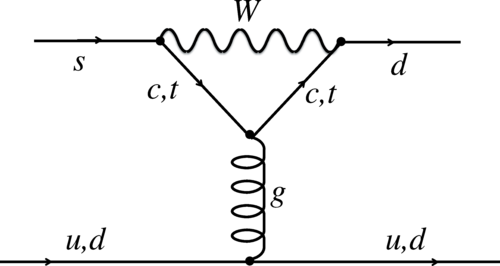
\includegraphics[width=0.9\textwidth]{3_loop_level.png} % first figure itself
        \end{minipage}\hfill
    \begin{minipage}{0.50\textwidth}
        \centering
        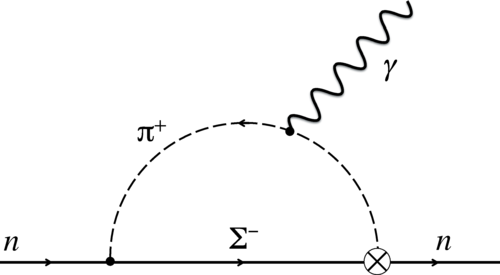
\includegraphics[width=0.9\textwidth]{chiral_loop.png} % second figure itself
        \end{minipage}
    \caption[The 3-loop level ``strong penguin'' diagram at the crossed-circle point of CP-odd meson-nucleon-nucleon interaction giving the effective SM CP-violation.]{The 3-loop level ``strong penguin'' diagram at the crossed-circle point of CP-odd meson-nucleon-nucleon interaction giving the effective SM CP-violation. Figure taken from \cite{Chupp2019}.}
    \label{fig:penguin}
\end{figure}
\clearpage}

\subsubsection{The strong sector:}
CP violation in the strong sector is also possible due to the $\Bar{\theta}$-term in the SM Quantum Chromodynamics (QCD) Lagrangian. 
\begin{equation}
    %\mathcal{L}=-\frac{1}{4}F_{\mu\nu}F^{\mu\nu}-\frac{n_fg^2\theta}{32\pi^2}F_{\mu\nu}\Tilde{F}^{\mu\nu}+\Bar{\psi}(i\gamma^\mu\mathcal{D}_\mu-me^{i\theta^{'}\gamma_5})\psi
    \mathcal{L}= \Bar{{\theta}}\frac{g^{2}_{s}}{32\pi^2}G^{a}_{\mu\nu}\Tilde{G}^{\mu\nu}_{a}
    \label{eq:qcd_theta}
\end{equation}
where $g_s$ is the strong force coupling constant and $G^{a}_{\mu\nu}$ and $\Tilde{G}^{\mu\nu}_{a}$ are the gluon field strength tensors, whose product violates CP symmetry \cite{Pospelov1999, Crewther1979}. Thus experimental constraints on nucleon nEDMs can be used to set upper limits on $\Bar{\theta}$ \cite{Pospelov1999, Crewther1979}. The nEDM in units of $\Bar{\theta}$ is given by:
\begin{equation}
    d_{n} \approx -(0.9 - 1.2) \times 10^{-16} \Bar{\theta} \; e \cdot cm
\end{equation}
so the current experimental limit implies $\Bar{\theta} \lesssim 10^{-10}$, neglecting hadronic uncertainties \cite{Seng2015}. This smallness of $\Bar{\theta}$ gives rise to the strong-CP problem. \cite{Peccei1977, Peccei1977a, Hooft1976a} propose a solution to this problem by introducing a global $U(1)$ chiral symmetry however, the breaking of such a symmetry leads to a new light pseudoscalar boson, called the axion. Although not yet observed, the axion is postulated to be a potential constituent candidate for dark matter with broad experimental efforts in search. 

%Furthermore, coupling of axion like particles to nucleons have been  The axion’s anomalous coupling to gluons induces, at energies below the confinement scale of QCD, a model-independent coupling of the axion to the operator giving rise to the EDM of the nucleon (N)

\subsection{nEDMs from Beyond the Standard Model}

Considering potential phenomena at energy scales well above the electroweak scale, BSM models proposed in \cite{Dubbers2011, Chupp1987} could introduce new CP and T violating interactions. Most of these BSM scenarios involve new particles with masses , $M_{BSM}$, well above the electroweak scale, giving rise to new couplings and further CP-violating phases, $\delta_{BSM}$ , which can, in principle, increase the magnitude of nEDM as (on a dimensional analysis basis) \cite{Alarcon2022, Chupp2019, Morrissey2012, Dubbers2011, Engel2013}: 
\begin{equation}
    d_{n} \sim 10^{-26}\; e \cdot cm\left(\frac{1~TeV}{M_{BSM}}\right)^2 \sin{\delta_{BSM}}
\end{equation}  
So far, measurements at the LHC have produced null results in searches for these BSM massive particles at 13 TeV energies \cite{PDG2022}. Since BSM predicted nEDM is, in principle, much larger than SM prediction, an improvement on the current nEDM limit can place constraints on CP violating BSM mass scales thus offering a complimentary probe to BSM searches at LHC. 

Considering the SM valid at low energy scales, the low energy manifestations of the possible high energy BSM physics can be described through an effective field theory (SMEFT) as:
\begin{equation}
    \mathcal{L}_{eff}^{CP} \approx \mathcal{L}_{SM} +  \underbrace{ \frac{ C^5 }{\Lambda} \mathcal{O}_i(5) + \sum_i \frac{ C_{i}^6 }{\Lambda^2} \mathcal{O}_i(6) + ... }_{\mathcal{L}_{BSM} }
\end{equation}
where $C_i$ encode all of short-distance information and $\Lambda$ is the effective BSM energy scale \cite{Chupp2019}. The leading CP violating operators, $\mathcal{O}_i$, which possibly contribute to nEDM, arise at dimension order six\footnote{Dimension-5 terms are only relevant for neutrino physics \cite{Agostini2023}.} and consist of quark EDMs, chromo-quark EDMs, chromo-gluon EDMs, CP-violating 3 gluon couplings, CP-violating four quark couplings and CP-violating quark-Higgs couplings \cite{Yamanaka2021}. These resulting effective CP-violating operators can be linked to an SMEFT that only contains the relevant hadronic physics and be solved for. Lattice QCD (LQCD) has shown promise to obtain ab initio QCD-based results. So far, LQCD has focused on calculating the nEDM from the quark EDMs and the QCD $\Bar{\theta}$ term in \cref{eq:qcd_theta} \cite{Alexandrou2021, Bhattacharya2021}. Higher-dimensional operators such as the quark and gluon chromo-EDMs are also being calculated. \cite{Shindler2021} provides a more thorough review of these approaches.
%(see Shindler [51] for a recent review , [27,28,46,47 in pdg]).

\subsection{Interpreting the nEDM}

Even though nEDM is a useful probe for CP violating physics, it is insufficient to explain the fundamental CP violating mechanism responsible for the baryon asymmetry problem. Further searches for the EDMs of multiple systems (quarks, leptons, nucleons, light nuclei, atoms and more) have to performed, along with their theoretical calculations, to understand the manifestation of fundamental CP violation in the effective energy hierarchy of these systems \footnote{As compared to other subatomic particles, experiments on free neutrons are a little less challenging to perform since neutrons are electrically neutral \cite{Chadwick1932} and thus, not influenced by electromagnetic fields, and they can be mass produced in reactors as well as spallation sources.} \cite{Chupp2019}. A schematic illustration of how EDMs can be used to search for fundamental CP violation sources is shown in \cref{fig:nEDM_Globalpic}. The collective analysis of the CP violation from EDMs as well as the CP violation from the CKM and PMNS sectors will provide a more global perspective on the true CP violating phenomena at the fundamental level. 

\afterpage{
\begin{figure}
    \centering
    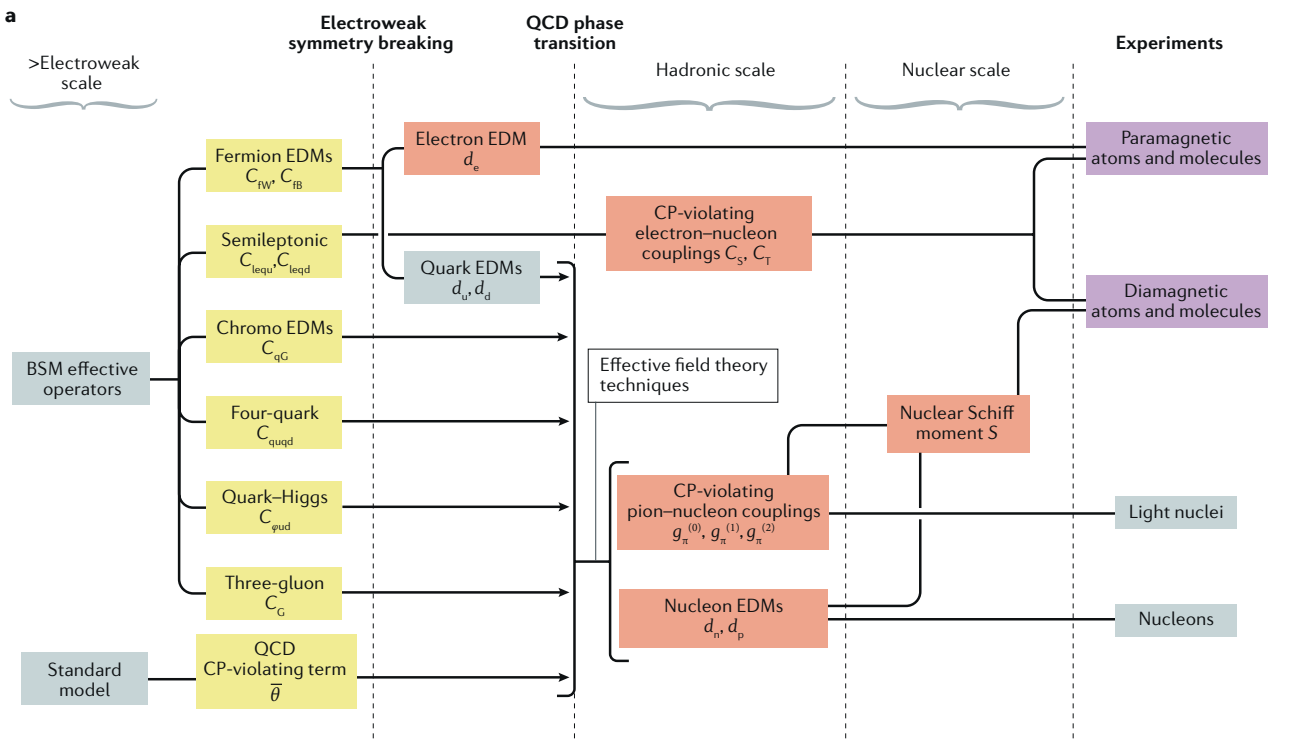
\includegraphics[width=\textwidth]{figures/chapter1-figs/EDM_interp2.png}
    \caption[A flow diagram illustrating the effective energy hierarchy based global analysis of fundamental BSM CP-violating interactions manifesting in observable low-energy CP-violating phenomena.]{A flow diagram illustrating the effective energy hierarchy based global analysis of fundamental BSM CP-violating interactions manifesting in observable low-energy CP-violating phenomena. Figure taken from \cite{Cairncross2019}.}
    \label{fig:nEDM_Globalpic}
\end{figure}
\clearpage}

\section{Principles of nEDM Measurement}

The primary method for measuring the nEDM is to look for a change in the Larmor precession frequency of neutrons, $\omega_n$, with a magnetic moment, $\mu_n$, and an electric dipole moment, $d_n$, under the application of a large static electric field, $E_0$, parallel and antiparallel with respect to a small static magnetic field, $B_0$ \cite{Ahmed2019}. This is illustrated in \cref{fig:Larmor} and can be stated as:
\begin{equation} \label{eq:larmor}
\omega_n=\frac{-2\left(\mu_n B_0\pm d_n E_0\right)}{\hbar}
\end{equation}
The statistical uncertainty of the nEDM measurement depends on the strength of the applied electric field, $E_0$, the number of neutrons observed, $N$, and the precession measurement time, $\tau$, \cite{Ahmed2019} as:
\begin{equation} \label{eq:uncertainty}
\sigma_{d_n}=\frac{\sqrt{2} \hbar}{4 E_0 \tau \sqrt{N}}
\end{equation}
The next generation of nEDM experiments aiming to improve upon nEDM limit optimize the quantity $ E_0 \tau \sqrt{N} $.

\afterpage{
\begin{figure}
    \centering
    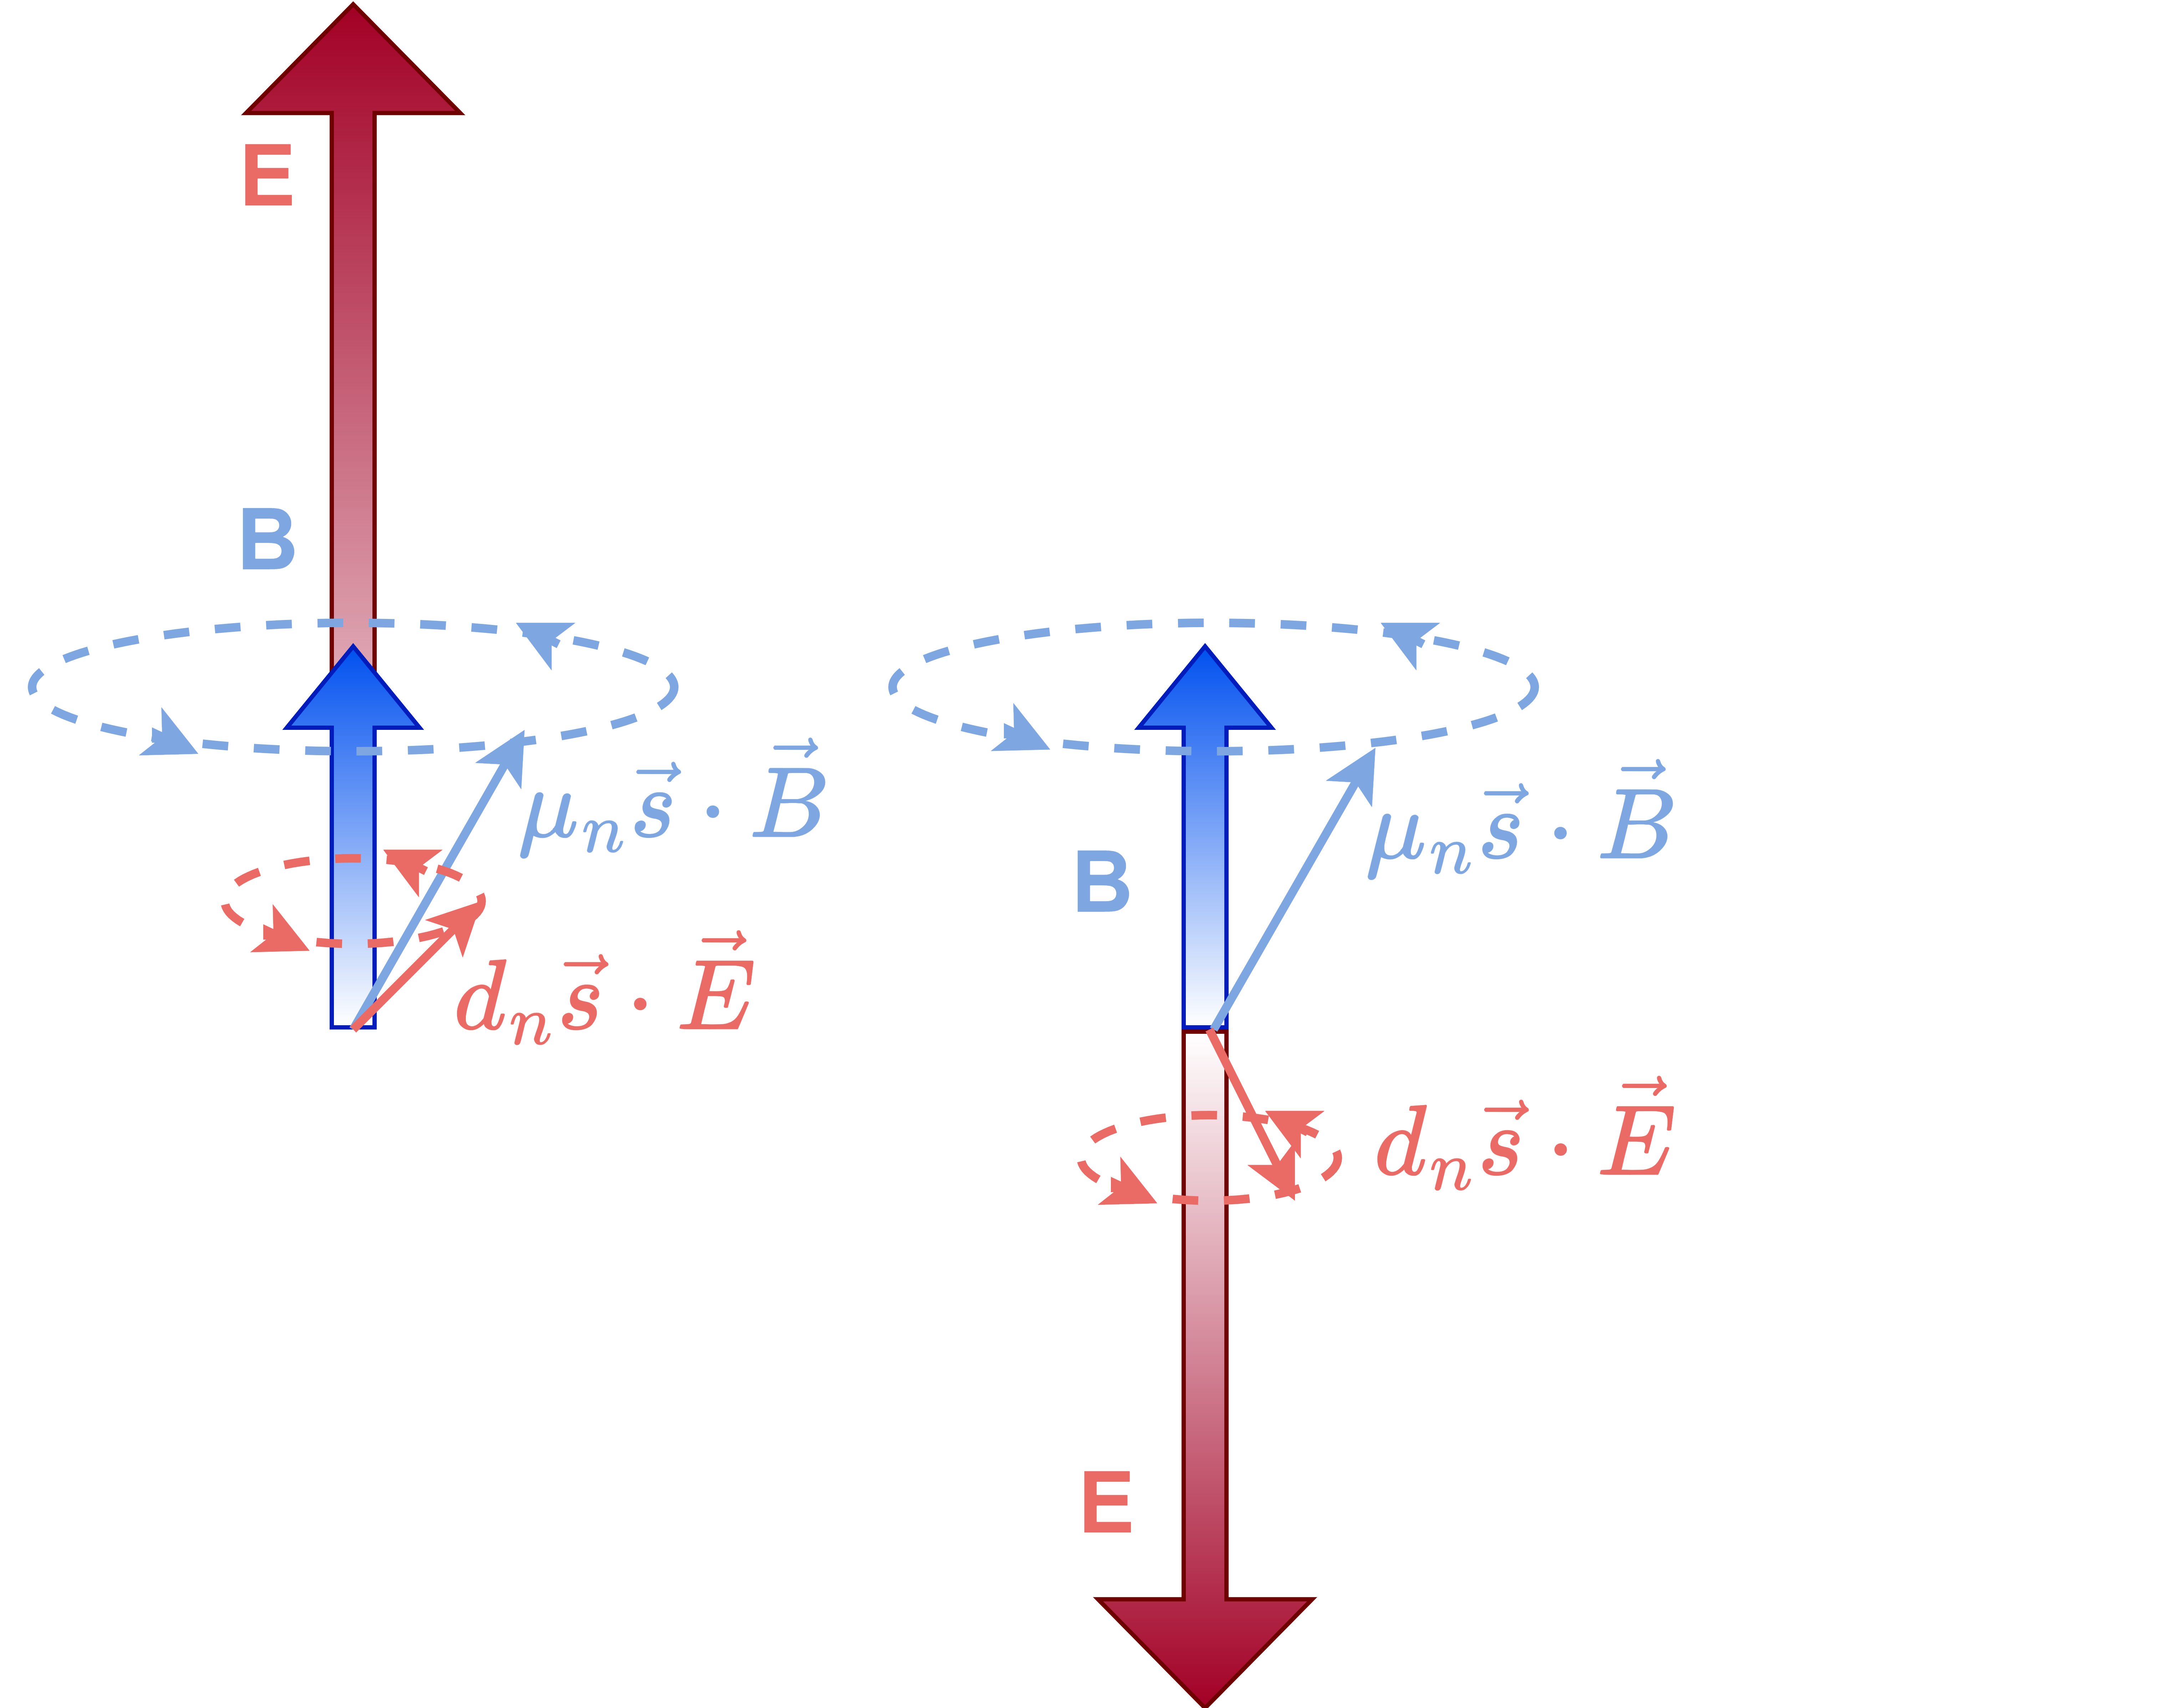
\includegraphics[width=0.75\textwidth]{figures/chapter1-figs/Larmor_precession.png}
    \caption[A cartoon illustrating the Larmor precesion of the neutron with a magnetic moment and an electric dipole moment under the application of an electric field, E, parallel and antiparallel with respect to a magnetic field, B.]{A cartoon illustrating the Larmor precesion of the neutron with a magnetic moment and an electric dipole moment under the application of an electric field, E, parallel and antiparallel with respect to a magnetic field, B.}
    \label{fig:Larmor}
\end{figure}
\clearpage}

The first experiment to look for nEDM took place at the neutron beam of the Oak ridge graphite reactor, where the nEDM from Larmor precession was measured using the method of separated oscillatory fields \cite{Ramsey1950, Purcell1950, Smith1957}. This neutron beam method has mostly been abandoned due to the discovery of a systematic effect associated with the motional magnetic field prohibiting the sensitivity reach towards the expected nEDM \cite{Dress1977}. Despite the large counting statistics advantage of neutron beams, these early measurements pointed out that competitive precision can be obtained with the slower Ultracold Neutrons (UCN), which can be stored for longer periods of time, and therefore, allow for a longer neutron precession measurements \cite{Golub1991}.

UCNs are essentially defined by the materials used to store them \cite{Golub1979a, Golub1991}. The interaction of UCN (Kinetic energy (K.E.) $\sim$ 200 neV, $\lambda$ $\sim$ 100~\AA, T $\sim$ mK) with material surfaces is characterized by an effective potential energy, $V_F$ , which is set by the coherent scattering length of neutrons from many nuclei in the storage material and is positive for most materials \cite{Fermi1936, Fermi1947, Golub1979a, Golub1991}. Neutrons with K.E. $<$  $V_F$ are repelled from the chamber walls, undergoing total external reflection and effectively getting confined \cite{Zeldovich1959, Steyerl1969, Lushchikov1969, Golub1979a,  Golub1991}. This storage allows for long precession and observation times of several hundred seconds and hence, precise measurements of nEDM \cite{Golub1991}.

Improving upon nEDM limit by optimizing the quantity $ E_0 \tau \sqrt{N} $ is difficult. Despite the storage advantage of UCNs, the limiting factor for nEDM sensitivity is achieving a high UCN density (UCN/cm$^3$). By employing the neutron superthermal scattering method from superfluid helium or solid deuterium, new UCN sources have been and are being developed for nEDM experiments to provide high UCN densities and hence high statistics \cite{Golub1975, Golub1979a, Golub1991}. The strength of the electric field is typically limited by the field emission electrons at the electrostatic boundaries of the electrodes. The precession time is limited from various UCN loss mechanisms with the UCN storage/transport material.

In natural units, the magnetic moment of neutron, $|\mu_n|$ = 0.332 GeV$^{-1}$ , is 14 orders of magnitude bigger then the most recent nEDM limit, $|d_n|$ $<$ 4.58 $\times$ 10$^{-15}$ GeV$^{-1}$ \cite{Codata2021, PDG2022}. To put that in perspective, the precession frequency from the neutron's magnetic moment in the 50 µT Earth’s magnetic field is around 250 Hz (corresponding to $10^{-12} eV$) while the current limit of nEDM $10^{-26}$ e$\cdot$cm in the 3 MV/m breakdown electric field of the Earth’s atmosphere causes a precession of 24 nHz (corresponding to $10^{-22} eV$). This illustrates that the precession signal from the magnetic interaction overwhelmingly dominates the precession from the nEDM. If the magnetic fields are kept highly uniform, the dominating magnetic interaction can be measured and accounted for. Therefore, nEDM experiments necessitate meticulous control of magnetic field fluctuations and utilize highly advanced magnetics (magnetic shielding and magnetic field coil geometries) and atomic comagnetometry (spin polarized species that occupy the same volume as the stored UCN, thus providing the a live average of the magnetic field experienced by the stored UCN) to monitor the stability and uniformity of the magnetic field \cite{Alarcon2022}. Nevertheless, this can only be done so well and systematic effects from magnetic field non-uniformities are bound to arise. The geometric phase effect, caused by the combination between non-uniformity of the magnetic field and the motional magnetic field, is, at present, the largest systematic effect limiting the nEDM sensitivity \cite{Pendlebury2004}.    

Improvements to UCN storage technology has been made for nEDM measurements at the Institut Laue-Langevin (ILL) \cite{Baker2006} and the Petersburg Nuclear Physics Institute (PNPI) \cite{Serebrov2014}. The most recent experimental limit  of $\mid d_n \mid < 1.8 \times 10^{-26}$ e$\cdot$cm (90\% C.L.) was set by the Paul Scherrer Institut (PSI) in 2020 \cite{Abel2020} using a room temperature ILL style separated oscillatory fields nEDM apparatus with an external UCN source and atomic magnetometry to account for the geometric phase systematic effect. The PSI nEDM experiment was able to achieve an average UCN density of 2 UCN/cm$^{-3}$, an electric field of 10 kV/cm and a precession time of $\sim$180 seconds. The historical advancement of the nEDM upper limit is shown in \cref{fig:nEDM_history}. The figure shows that further experimental searches are needed to push the upper limit of the nEDM in order to constraint BSM predictions.  

\afterpage{
\begin{figure}
    \centering
    \includegraphics[width=\textwidth]{figures/chapter1-figs/nEDMupperbounds_3.png}
    \caption[A history plot of the measured nEDM upper limits.]{A history plot of the measured nEDM upper limits. The colored regions show the nEDM predicted values from the SM and BSM predictions \cite{Chupp2019}. Some key nEDM experiments throoughout history are highlighted. The latest upper limit measured in and 2020\cite{Abel2020} is also shown. The horizontal green line indicates the projected goal of nEDM@SNS experiment \cite{Ahmed2019}. A more complete list of all the nEDM experiments performed so far can be found in \cite{Lamoreaux2009} and \cite{PDG2022}.}
    \label{fig:nEDM_history}
\end{figure}
\clearpage}

\section{Outline of Dissertation}

This chapter impresses the need for new searches of CP violating phenomena to explain the baryon asymmetry of the universe. The chapter also describes how the nEDM is a powerful CP violating phenomena that can perhaps elucidate the baryon asymmetry problem. Now that the physics is well motivated, a new experimental search along with an the associated R\&D project are described in the following chapters:
\begin{itemize}
    \item \Cref{ch:nEDM} describes the nEDM@SNS experiment, which aims to reach a nEDM sensitivity of a few $\times~10^{-28}$ e$\cdot$cm. In this experiment, polarized UCNs, polarized $^3$He in a solution of superfluid $^4$He will used \cite{Ahmed2019}. Technical details about the innovative measurement techniques as well as the experimental apparatus design are discussed.
    \item \Cref{ch:polHe} describes the neutron polarimetry technique, where polarized $^3$He is used to perform neutron spin polarization analysis. The first half of the chapter is dedicated to the optical pumping techniques used to polarize $^3$He and the latter half is describes the design and proof of demonstration of an in situ polarized $^3$He system for neutron spin analysis.   
    \item \Cref{ch:PT} describes the neutron polarization and transmission measurements, a preliminary R\&D effort, to verify the design of the cryomagnet of the nEDM@SNS experiment. The uniaxial neutron polarimetry experimental setup at the monochromatic neutron SNS beamline 13A is presented followed by results of the data taking campaign in the summer of 2023. Lastly, Small Angle Neutron Scattering measurements on the beam windows materials are presented.   
    \item \Cref{ch:conclusions} briefly summarises and discusses the main neutron polarization and transmission results detailed in this dissertation and then presents future plans for an upgraded setup.
\end{itemize}